% Options for packages loaded elsewhere
% Options for packages loaded elsewhere
\PassOptionsToPackage{unicode}{hyperref}
\PassOptionsToPackage{hyphens}{url}
\PassOptionsToPackage{dvipsnames,svgnames,x11names}{xcolor}
%
\documentclass[
  11pt,
  ignorenonframetext,
]{beamer}
\geometry{left = 10mm,right = 10mm}
\newif\ifbibliography
\usepackage{pgfpages}
\setbeamertemplate{caption}[numbered]
\setbeamertemplate{caption label separator}{: }
\setbeamercolor{caption name}{fg=normal text.fg}
\beamertemplatenavigationsymbolshorizontal
% remove section numbering
\setbeamertemplate{part page}{
  \centering
  \begin{beamercolorbox}[sep=16pt,center]{part title}
    \usebeamerfont{part title}\insertpart\par
  \end{beamercolorbox}
}
\setbeamertemplate{section page}{
  \centering
  \begin{beamercolorbox}[sep=12pt,center]{section title}
    \usebeamerfont{section title}\insertsection\par
  \end{beamercolorbox}
}
\setbeamertemplate{subsection page}{
  \centering
  \begin{beamercolorbox}[sep=8pt,center]{subsection title}
    \usebeamerfont{subsection title}\insertsubsection\par
  \end{beamercolorbox}
}
% Prevent slide breaks in the middle of a paragraph
\widowpenalties 1 10000
\raggedbottom
\AtBeginPart{
  \frame{\partpage}
}
\AtBeginSection{
  \ifbibliography
  \else
    \frame{\sectionpage}
  \fi
}
\AtBeginSubsection{
  \frame{\subsectionpage}
}
\usepackage{iftex}
\ifPDFTeX
  \usepackage[T1]{fontenc}
  \usepackage[utf8]{inputenc}
  \usepackage{textcomp} % provide euro and other symbols
\else % if luatex or xetex
  \usepackage{unicode-math} % this also loads fontspec
  \defaultfontfeatures{Scale=MatchLowercase}
  \defaultfontfeatures[\rmfamily]{Ligatures=TeX,Scale=1}
\fi
\usepackage{lmodern}

\usetheme[]{Berlin}
\usecolortheme[]{lily}
\usefonttheme{serif} % use mainfont rather than sansfont for slide text
\ifPDFTeX\else
  % xetex/luatex font selection
  \setmainfont[]{Calibri}
\fi
% Use upquote if available, for straight quotes in verbatim environments
\IfFileExists{upquote.sty}{\usepackage{upquote}}{}
\IfFileExists{microtype.sty}{% use microtype if available
  \usepackage[]{microtype}
  \UseMicrotypeSet[protrusion]{basicmath} % disable protrusion for tt fonts
}{}
\makeatletter
\@ifundefined{KOMAClassName}{% if non-KOMA class
  \IfFileExists{parskip.sty}{%
    \usepackage{parskip}
  }{% else
    \setlength{\parindent}{0pt}
    \setlength{\parskip}{6pt plus 2pt minus 1pt}}
}{% if KOMA class
  \KOMAoptions{parskip=half}}
\makeatother


\usepackage{longtable,booktabs,array}
\usepackage{calc} % for calculating minipage widths
\usepackage{caption}
% Make caption package work with longtable
\makeatletter
\def\fnum@table{\tablename~\thetable}
\makeatother
\usepackage{graphicx}
\makeatletter
\newsavebox\pandoc@box
\newcommand*\pandocbounded[1]{% scales image to fit in text height/width
  \sbox\pandoc@box{#1}%
  \Gscale@div\@tempa{\textheight}{\dimexpr\ht\pandoc@box+\dp\pandoc@box\relax}%
  \Gscale@div\@tempb{\linewidth}{\wd\pandoc@box}%
  \ifdim\@tempb\p@<\@tempa\p@\let\@tempa\@tempb\fi% select the smaller of both
  \ifdim\@tempa\p@<\p@\scalebox{\@tempa}{\usebox\pandoc@box}%
  \else\usebox{\pandoc@box}%
  \fi%
}
% Set default figure placement to htbp
\def\fps@figure{htbp}
\makeatother


% definitions for citeproc citations
\NewDocumentCommand\citeproctext{}{}
\NewDocumentCommand\citeproc{mm}{%
  \begingroup\def\citeproctext{#2}\cite{#1}\endgroup}
\makeatletter
 % allow citations to break across lines
 \let\@cite@ofmt\@firstofone
 % avoid brackets around text for \cite:
 \def\@biblabel#1{}
 \def\@cite#1#2{{#1\if@tempswa , #2\fi}}
\makeatother
\newlength{\cslhangindent}
\setlength{\cslhangindent}{1.5em}
\newlength{\csllabelwidth}
\setlength{\csllabelwidth}{3em}
\newenvironment{CSLReferences}[2] % #1 hanging-indent, #2 entry-spacing
 {\begin{list}{}{%
  \setlength{\itemindent}{0pt}
  \setlength{\leftmargin}{0pt}
  \setlength{\parsep}{0pt}
  % turn on hanging indent if param 1 is 1
  \ifodd #1
   \setlength{\leftmargin}{\cslhangindent}
   \setlength{\itemindent}{-1\cslhangindent}
  \fi
  % set entry spacing
  \setlength{\itemsep}{#2\baselineskip}}}
 {\end{list}}
\usepackage{calc}
\newcommand{\CSLBlock}[1]{\hfill\break\parbox[t]{\linewidth}{\strut\ignorespaces#1\strut}}
\newcommand{\CSLLeftMargin}[1]{\parbox[t]{\csllabelwidth}{\strut#1\strut}}
\newcommand{\CSLRightInline}[1]{\parbox[t]{\linewidth - \csllabelwidth}{\strut#1\strut}}
\newcommand{\CSLIndent}[1]{\hspace{\cslhangindent}#1}



\setlength{\emergencystretch}{3em} % prevent overfull lines

\providecommand{\tightlist}{%
  \setlength{\itemsep}{0pt}\setlength{\parskip}{0pt}}



 


\usepackage{amssymb} % http://ctan.org/pkg/amssymb
\usepackage{pifont} % http://ctan.org/pkg/pifont

\makeatother



\makeatletter
\setbeamertemplate{headline}{
  \begin{beamercolorbox}[colsep=1.5pt]{upper separation line head}
  \end{beamercolorbox}
  \begin{beamercolorbox}{section in head/foot}
  \vskip2pt\insertnavigation{\paperwidth}\vskip2pt
  \end{beamercolorbox}%
  \begin{beamercolorbox}[colsep=1.5pt]{lower separation line head}
  \end{beamercolorbox}
}
\makeatother

\setbeamertemplate{footline}{
  \leavevmode%
  \hbox{%
    \begin{beamercolorbox}[wd=0.4\paperwidth,ht=2.25ex,dp=1ex,center]{author in head/foot}%
    \usebeamerfont{author in head/foot}\insertshortauthor
    \end{beamercolorbox}%
    \begin{beamercolorbox}[wd=0.525\paperwidth,ht=2.25ex,dp=1ex,center]{shorttitle in head/foot}%
    \usebeamerfont{shorttitle in head/foot}\insertshorttitle
    \end{beamercolorbox}%
    \begin{beamercolorbox}[wd=0.075\paperwidth,ht=2.25ex,dp=1ex,right]{slide in head/foot}%
    \insertframenumber{} / \inserttotalframenumber\hspace*{2ex} 
    \end{beamercolorbox}%
  }%
  \vskip0pt%
}
\makeatother

% Make Slide Area Larger
\setbeamersize{
  text margin left    = .04\paperwidth,
  text margin right   = .04\paperwidth
}

\makeatletter
\newcommand\disablecolorlinks{\def\HyColor@UseColor##1{}}
\makeatletter
\addtobeamertemplate{headline}{\disablecolorlinks{}}{}
\usepackage{booktabs}
\usepackage{longtable}
\usepackage{array}
\usepackage{multirow}
\usepackage{wrapfig}
\usepackage{float}
\usepackage{colortbl}
\usepackage{pdflscape}
\usepackage{tabu}
\usepackage{threeparttable}
\usepackage{threeparttablex}
\usepackage[normalem]{ulem}
\usepackage{makecell}
\usepackage{xcolor}
\makeatletter
\@ifpackageloaded{caption}{}{\usepackage{caption}}
\AtBeginDocument{%
\ifdefined\contentsname
  \renewcommand*\contentsname{Table of contents}
\else
  \newcommand\contentsname{Table of contents}
\fi
\ifdefined\listfigurename
  \renewcommand*\listfigurename{List of Figures}
\else
  \newcommand\listfigurename{List of Figures}
\fi
\ifdefined\listtablename
  \renewcommand*\listtablename{List of Tables}
\else
  \newcommand\listtablename{List of Tables}
\fi
\ifdefined\figurename
  \renewcommand*\figurename{Figure}
\else
  \newcommand\figurename{Figure}
\fi
\ifdefined\tablename
  \renewcommand*\tablename{Table}
\else
  \newcommand\tablename{Table}
\fi
}
\@ifpackageloaded{float}{}{\usepackage{float}}
\floatstyle{ruled}
\@ifundefined{c@chapter}{\newfloat{codelisting}{h}{lop}}{\newfloat{codelisting}{h}{lop}[chapter]}
\floatname{codelisting}{Listing}
\newcommand*\listoflistings{\listof{codelisting}{List of Listings}}
\makeatother
\makeatletter
\makeatother
\makeatletter
\@ifpackageloaded{caption}{}{\usepackage{caption}}
\@ifpackageloaded{subcaption}{}{\usepackage{subcaption}}
\makeatother

\usepackage{bookmark}
\IfFileExists{xurl.sty}{\usepackage{xurl}}{} % add URL line breaks if available
\urlstyle{same}
% Make links footnotes instead of hotlinks:
\DeclareRobustCommand{\href}[2]{#2\footnote{\url{#1}}}
\hypersetup{
  pdftitle={Long Title That is Meant Only For The Title Slide},
  pdfauthor={First Author1; Other Author2},
  colorlinks=true,
  linkcolor={blue},
  filecolor={Maroon},
  citecolor={Blue},
  urlcolor={Blue},
  pdfcreator={LaTeX via pandoc}}


\title[A Shorter Title]{Long Title That is Meant Only For The Title
Slide}
\subtitle{A Subtitle for the Presentation}
\author{First Author\textsuperscript{1} \and Other
Author\textsuperscript{2}}
\date{2024-10-24}
\institute{\textsuperscript{1}Department of Domain,\\
University of Institution School of School\\
City, State, Country \and \textsuperscript{2}Department of
Affiliation,\\
Other University\\
City, State, Country}

\begin{document}
\frame{\titlepage}


\section{Equations and Plots}\label{equations-and-plots}

\begin{frame}{Example of In-Line and Display Equations}
\phantomsection\label{example-of-in-line-and-display-equations}
\begin{itemize}
\tightlist
\item
  Content for the first slide
\item
  In-Line Equation: \(E[Y \vert X ] = \beta_{0} + \beta_{x}X\)
\end{itemize}

\[ y_{i} = \beta_{0} + \sum_{j=1}^{p}X_{ij} + \epsilon_{i}\]
\end{frame}

\begin{frame}{Here's a Table Using \texttt{table1::table1()}}
\phantomsection\label{heres-a-table-using-table1table1}
\begin{table}
\centering
\begin{tabular}[b]{>{}c|>{}c|>{}c|c}
\hline
\textbf{ } & \textbf{0. V-shaped} & \textbf{1. Straight} & \textbf{Overall}\\
\hline
\begingroup\fontsize{7}{9}\selectfont \cellcolor{gray!10}{}\endgroup & \begingroup\fontsize{7}{9}\selectfont \cellcolor{gray!10}{(N=18)}\endgroup & \begingroup\fontsize{7}{9}\selectfont \cellcolor{gray!10}{(N=14)}\endgroup & \begingroup\fontsize{7}{9}\selectfont \cellcolor{gray!10}{(N=32)}\endgroup\\
\hline
\textbf{\begingroup\fontsize{7}{9}\selectfont Fuel Efficiency: Miles/(US) Gallon\endgroup} & \textbf{\begingroup\fontsize{7}{9}\selectfont \endgroup} & \textbf{\begingroup\fontsize{7}{9}\selectfont \endgroup} & \textbf{\begingroup\fontsize{7}{9}\selectfont \endgroup}\\
\hline
\begingroup\fontsize{7}{9}\selectfont \cellcolor{gray!10}{Mean (SD)}\endgroup & \begingroup\fontsize{7}{9}\selectfont \cellcolor{gray!10}{16.6 (3.86)}\endgroup & \begingroup\fontsize{7}{9}\selectfont \cellcolor{gray!10}{24.6 (5.38)}\endgroup & \begingroup\fontsize{7}{9}\selectfont \cellcolor{gray!10}{20.1 (6.03)}\endgroup\\
\hline
\begingroup\fontsize{7}{9}\selectfont Median [Min, Max]\endgroup & \begingroup\fontsize{7}{9}\selectfont 15.7 [10.4, 26.0]\endgroup & \begingroup\fontsize{7}{9}\selectfont 22.8 [17.8, 33.9]\endgroup & \begingroup\fontsize{7}{9}\selectfont 19.2 [10.4, 33.9]\endgroup\\
\hline
\textbf{\begingroup\fontsize{7}{9}\selectfont \cellcolor{gray!10}{Displacement (in\textasciicircum{}3)}\endgroup} & \textbf{\begingroup\fontsize{7}{9}\selectfont \cellcolor{gray!10}{}\endgroup} & \textbf{\begingroup\fontsize{7}{9}\selectfont \cellcolor{gray!10}{}\endgroup} & \textbf{\begingroup\fontsize{7}{9}\selectfont \cellcolor{gray!10}{}\endgroup}\\
\hline
\begingroup\fontsize{7}{9}\selectfont Mean (SD)\endgroup & \begingroup\fontsize{7}{9}\selectfont 307 (107)\endgroup & \begingroup\fontsize{7}{9}\selectfont 132 (56.9)\endgroup & \begingroup\fontsize{7}{9}\selectfont 231 (124)\endgroup\\
\hline
\begingroup\fontsize{7}{9}\selectfont \cellcolor{gray!10}{Median [Min, Max]}\endgroup & \begingroup\fontsize{7}{9}\selectfont \cellcolor{gray!10}{311 [120, 472]}\endgroup & \begingroup\fontsize{7}{9}\selectfont \cellcolor{gray!10}{121 [71.1, 258]}\endgroup & \begingroup\fontsize{7}{9}\selectfont \cellcolor{gray!10}{196 [71.1, 472]}\endgroup\\
\hline
\textbf{\begingroup\fontsize{7}{9}\selectfont Gross Horsepower\endgroup} & \textbf{\begingroup\fontsize{7}{9}\selectfont \endgroup} & \textbf{\begingroup\fontsize{7}{9}\selectfont \endgroup} & \textbf{\begingroup\fontsize{7}{9}\selectfont \endgroup}\\
\hline
\begingroup\fontsize{7}{9}\selectfont \cellcolor{gray!10}{Mean (SD)}\endgroup & \begingroup\fontsize{7}{9}\selectfont \cellcolor{gray!10}{190 (60.3)}\endgroup & \begingroup\fontsize{7}{9}\selectfont \cellcolor{gray!10}{91.4 (24.4)}\endgroup & \begingroup\fontsize{7}{9}\selectfont \cellcolor{gray!10}{147 (68.6)}\endgroup\\
\hline
\begingroup\fontsize{7}{9}\selectfont Median [Min, Max]\endgroup & \begingroup\fontsize{7}{9}\selectfont 180 [91.0, 335]\endgroup & \begingroup\fontsize{7}{9}\selectfont 96.0 [52.0, 123]\endgroup & \begingroup\fontsize{7}{9}\selectfont 123 [52.0, 335]\endgroup\\
\hline
\end{tabular}
\end{table}
\end{frame}

\begin{frame}{Here's A Plot: Palette 1 - Lancet}
\phantomsection\label{heres-a-plot-palette-1---lancet}
\begin{center}
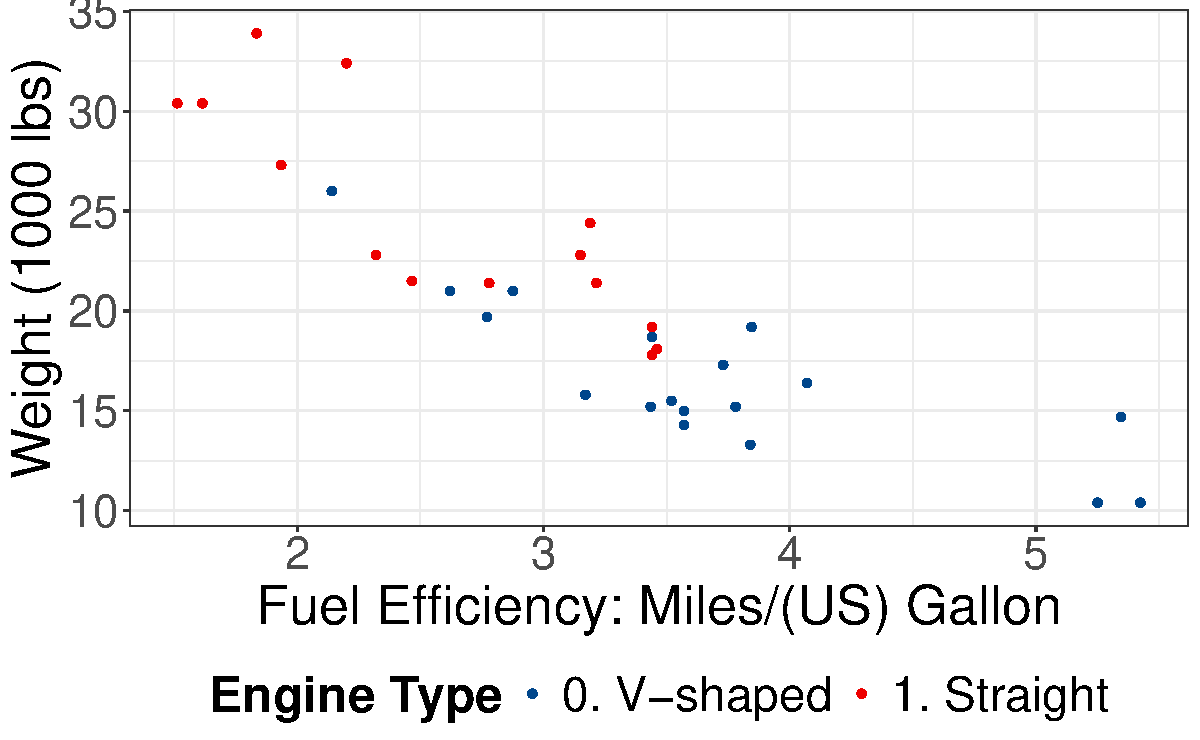
\includegraphics[width=\linewidth,height=0.8\textheight,keepaspectratio]{figures/mtcars-scatter-mpg-by-wt-palette-1-1.pdf}
\end{center}
\end{frame}

\begin{frame}{Here's A Plot: Palette 2 - NEJM}
\phantomsection\label{heres-a-plot-palette-2---nejm}
\begin{center}
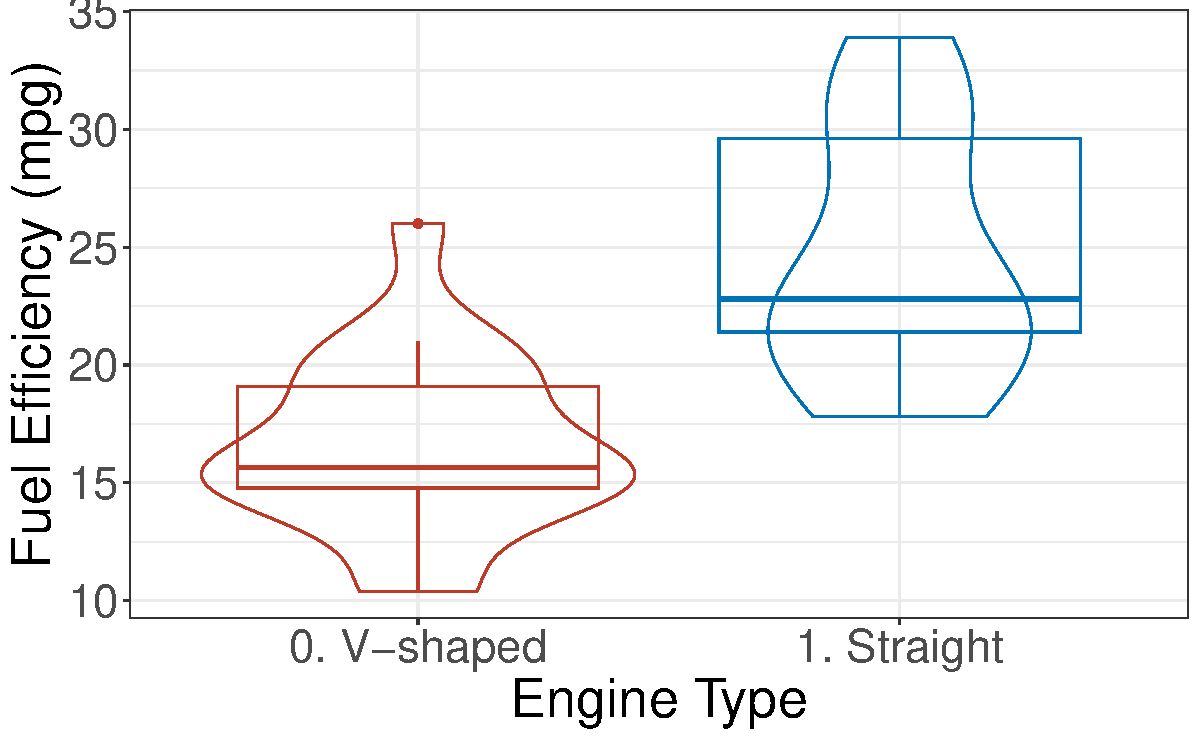
\includegraphics[width=\linewidth,height=0.8\textheight,keepaspectratio]{figures/mtcars-boxplot-mpg-by-vs-palette-2-1.pdf}
\end{center}
\end{frame}

\begin{frame}{Here's A Plot: Palette 3 - BMJ}
\phantomsection\label{heres-a-plot-palette-3---bmj}
\begin{center}
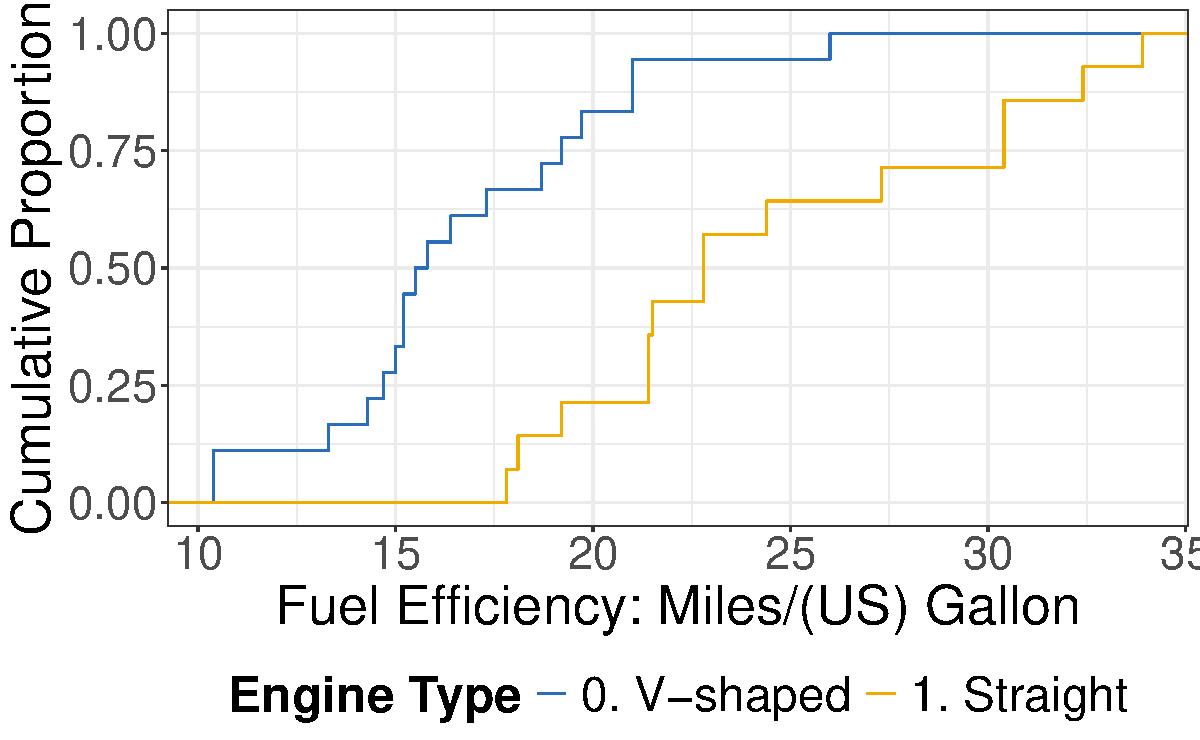
\includegraphics[width=\linewidth,height=0.8\textheight,keepaspectratio]{figures/mtcars-ecdf-mpg-by-vs-palette-3-1.pdf}
\end{center}
\end{frame}

\begin{frame}{Here's A Plot: Palette 3 - BMJ}
\phantomsection\label{heres-a-plot-palette-3---bmj-1}
\begin{center}
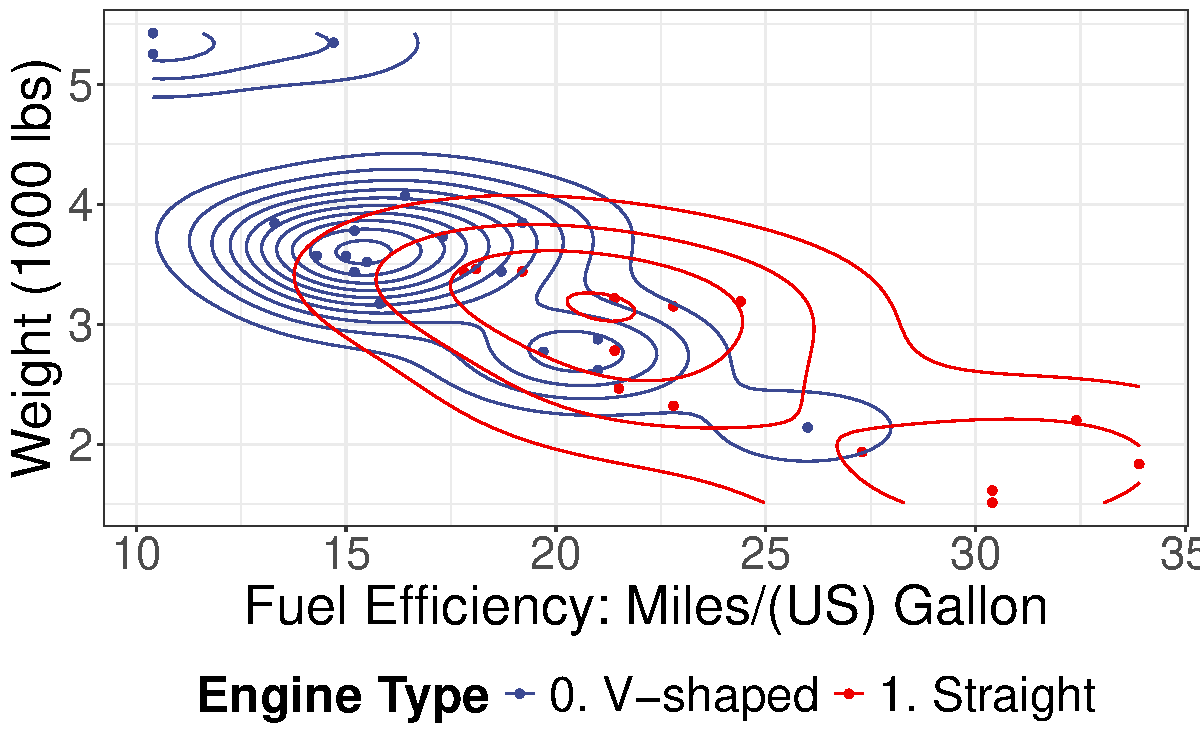
\includegraphics[width=\linewidth,height=0.8\textheight,keepaspectratio]{figures/mtcars-density-mpg-vs-wt-by-vs-palette-4-1.pdf}
\end{center}
\end{frame}

\section{Citations}\label{citations}

\begin{frame}[fragile]{Bibliography}
\phantomsection\label{bibliography}
\begin{itemize}
\tightlist
\item
  The bibliography is created by \texttt{bibliography.bib}
\item
  This is a \href{https://www.bibtex.org/}{bibtex file}
\item
  If you have an article DOI, convert it to bibtex with
  \href{https://www.doi2bib.org/}{DOI2Bib}
\item
  \href{https://quarto.org/docs/authoring/citations.html}{Citing are
  easy}: (\citeproc{ref-Xie2018RMarkdown}{Xie et al. 2018})
\item
  Customize with a \href{https://citationstyles.org/}{CSL File}

  \begin{itemize}
  \tightlist
  \item
    \href{https://github.com/citation-style-language/styles}{Link to
    Repository}
  \item
    This uses ASA's CSL.
  \end{itemize}
\end{itemize}
\end{frame}

\section{Incremental}\label{incremental}

\begin{frame}{More Content}
\phantomsection\label{more-content}
\begin{itemize}
\tightlist
\item
  This is yet another slide

  \begin{itemize}
  \tightlist
  \item
    Indented content
  \end{itemize}
\end{itemize}

\pause

\begin{itemize}
\tightlist
\item
  More Content
\end{itemize}

\pause

\begin{itemize}
\tightlist
\item
  Even More Content
\end{itemize}
\end{frame}

\section{References}\label{references}

\begin{frame}[allowframebreaks]{References}
\phantomsection\label{references-1}
\phantomsection\label{refs}
\begin{CSLReferences}{1}{0}
\bibitem[\citeproctext]{ref-Xie2018RMarkdown}
Xie, Y., Allaire, J. J., and Grolemund, G. (2018), \emph{R markdown: The
definitive guide}, Chapman; Hall/CRC.
\url{https://doi.org/10.1201/9781138359444}.

\end{CSLReferences}
\end{frame}




\end{document}
